\documentclass[a4paper]{article}
\usepackage[T1]{fontenc}
\usepackage[russian]{babel}
\usepackage[pdftex]{graphicx}
\usepackage[ruled,vlined]{algorithm2e}
\usepackage[utf8]{inputenc}
\usepackage{xcolor}
\usepackage{hyperref}
\usepackage{amsmath}
\usepackage{geometry}
\usepackage{float}
\usepackage{caption}
\usepackage{subcaption}
\DeclareGraphicsExtensions{.pdf,.png,.jpg}


\begin{document}

    \begin{titlepage}
        \Large
        \begin{center}
            Санкт-Петербургский \ Политехнический университет Петра Великого\\
            \vspace{10em}Отчет по лабораторной работе №3\\
            \vspace{2em}
            \textbf{Линейная регрессия}
        \end{center}
        \vspace{6em}
        \hfill\parbox{10cm}{
            \hspace*{2cm}\hspace*{-4cm}Студент:\hfill Швачко Никита Андреевич\\
            \hspace*{2cm}\hspace*{-4cm}Преподаватель:\hfill Баженов Александр Николаевич\\
            \hspace*{2cm}\hspace*{-4cm}Группа:\hfill 5030102/20202
        }
        \vspace{\fill}
        \begin{center}
            Санкт-Петербург \ 2025
        \end{center}
    \end{titlepage}



    \section{Постановка задачи}

    Целью лабораторной работы является изучение устойчивости различных методов оценки коэффициентов простой линейной регрессии к выбросам. Рассматривается модель:

    \begin{equation}
        y_i = \beta_0 + \beta_1 x_i + \varepsilon_i, \quad i=1,\ldots,n,
    \end{equation}

    где $x_i$ — заданные значения фактора, $y_i$ — значения отклика, $\varepsilon_i \sim N(0,1)$ — случайная ошибка. В качестве истинной зависимости используется:

    \begin{equation}
        y_i = 2 + 2x_i + \varepsilon_i.
    \end{equation}

    Оцениваются параметры $\beta_0$, $\beta_1$ двумя методами:
    \begin{itemize}
        \item методом наименьших квадратов (МНК);
        \item методом наименьших модулей (МНМ).
    \end{itemize}

    Для анализа устойчивости оценок в данные вносятся выбросы в первую и последнюю точки: $y_1 := y_1 + 10$, $y_{20} := y_{20} - 10$.


    \section{Описание используемых методов}

    \subsection{Метод наименьших квадратов (МНК)}

    Метод МНК минимизирует сумму квадратов отклонений модели от наблюдаемых данных:

    \begin{equation}
        Q(\beta_0, \beta_1) = \sum_{i=1}^n (y_i - \beta_0 - \beta_1 x_i)^2 \rightarrow \min_{\beta_0, \beta_1}.
    \end{equation}

    Оценки параметров находятся по формулам:

    \begin{equation}
        \hat{\beta}_1 = \frac{\overline{xy} - \bar{x}\bar{y}}{\overline{x^2} - \bar{x}^2}, \quad \hat{\beta}_0 = \bar{y} - \hat{\beta}_1 \bar{x}.
    \end{equation}

    \subsection{Метод наименьших модулей (МНМ)}

    МНМ минимизирует сумму модулей отклонений:

    \begin{equation}
        \sum_{i=1}^{n}|y_i - \beta_0 - \beta_1 x_i| \rightarrow \min_{\beta_0, \beta_1}.
    \end{equation}

    Оценки параметров вычисляются по формулам:

    \begin{equation}
        \hat{\beta}_{1R} = r_Q \cdot \frac{q_y^*}{q_x^*}, \quad \hat{\beta}_{0R} = \operatorname{med} y - \hat{\beta}_{1R} \cdot \operatorname{med} x,
    \end{equation}

    где $r_Q$ — робастная корреляция знаков, $q_x^*, q_y^*$ — интерквартильные размахи, вычисляемые с нормировкой $k_q(n)$.


    \section{Результаты эксперимента}

    Генерируются $n=20$ точек $x_i$ на отрезке $[-1.8; 2]$ с равномерным шагом $0.2$, ошибка $\varepsilon_i \sim N(0, 1)$. Полученные оценки параметров представлены ниже.

    \subsection*{Таблица 1: Невозмущённая выборка}

    \begin{table}[H]
        \centering
        \begin{tabular}{|c|c|c|c|c|c|}
            \hline
            & Метод & $\hat{a}$ & $\hat{a}/a$ & $\hat{b}$ & $\hat{b}/b$ \\
            \hline
            1 & МНК   & 2.60      & 1.30        & 1.70      & 0.85        \\
            2 & МНМ   & 2.31      & 1.16        & 1.64      & 0.82        \\
            \hline
        \end{tabular}
        \caption{Оценки коэффициентов регрессии без выбросов}
    \end{table}

    \subsection*{Таблица 2: Возмущённая выборка}

    \begin{table}[H]
        \centering
        \begin{tabular}{|c|c|c|c|c|c|}
            \hline
            & Метод & $\hat{a}$ & $\hat{a}/a$ & $\hat{b}$ & $\hat{b}/b$ \\
            \hline
            1 & МНК   & 2.74      & 1.37        & 0.27      & 0.14        \\
            2 & МНМ   & 2.35      & 1.17        & 1.31      & 0.65        \\
            \hline
        \end{tabular}
        \caption{Оценки коэффициентов регрессии с выбросами}
    \end{table}


    \section{Графики результатов}

    \begin{figure}[H]
        \centering
        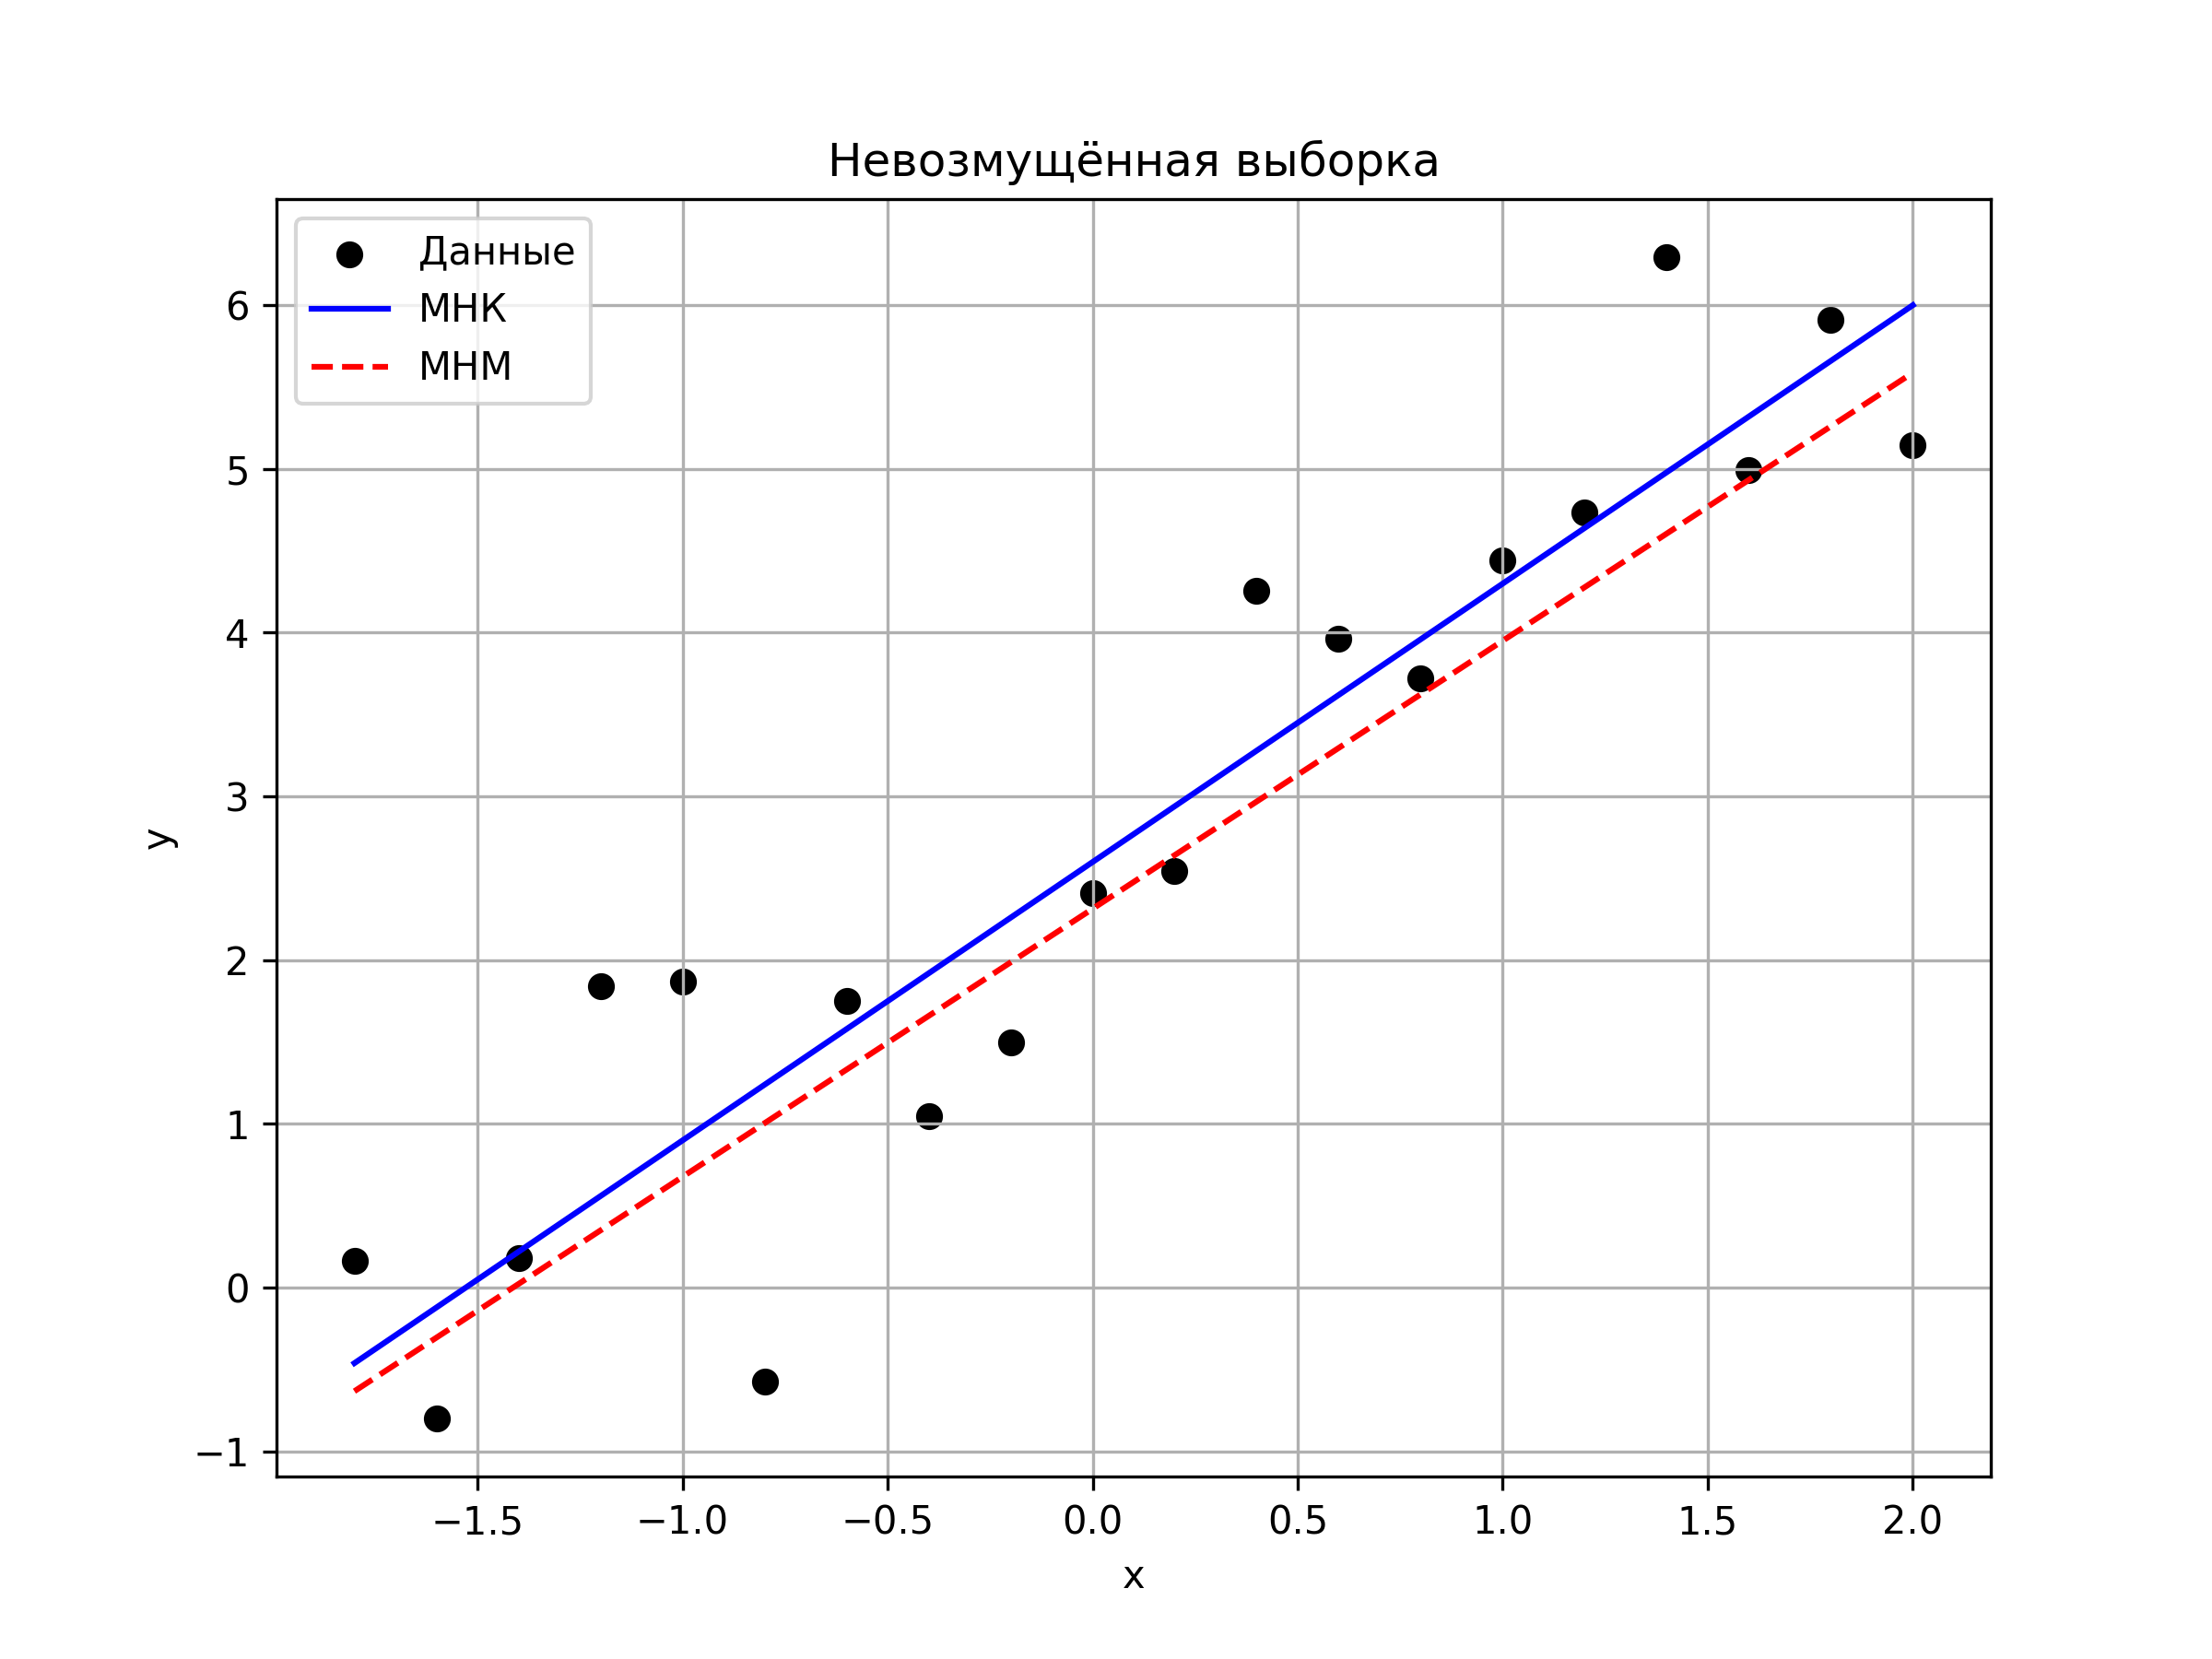
\includegraphics[width=0.8\textwidth]{regression_clean}
        \caption{Невозмущённая выборка: МНК и МНМ}
    \end{figure}

    \begin{figure}[H]
        \centering
        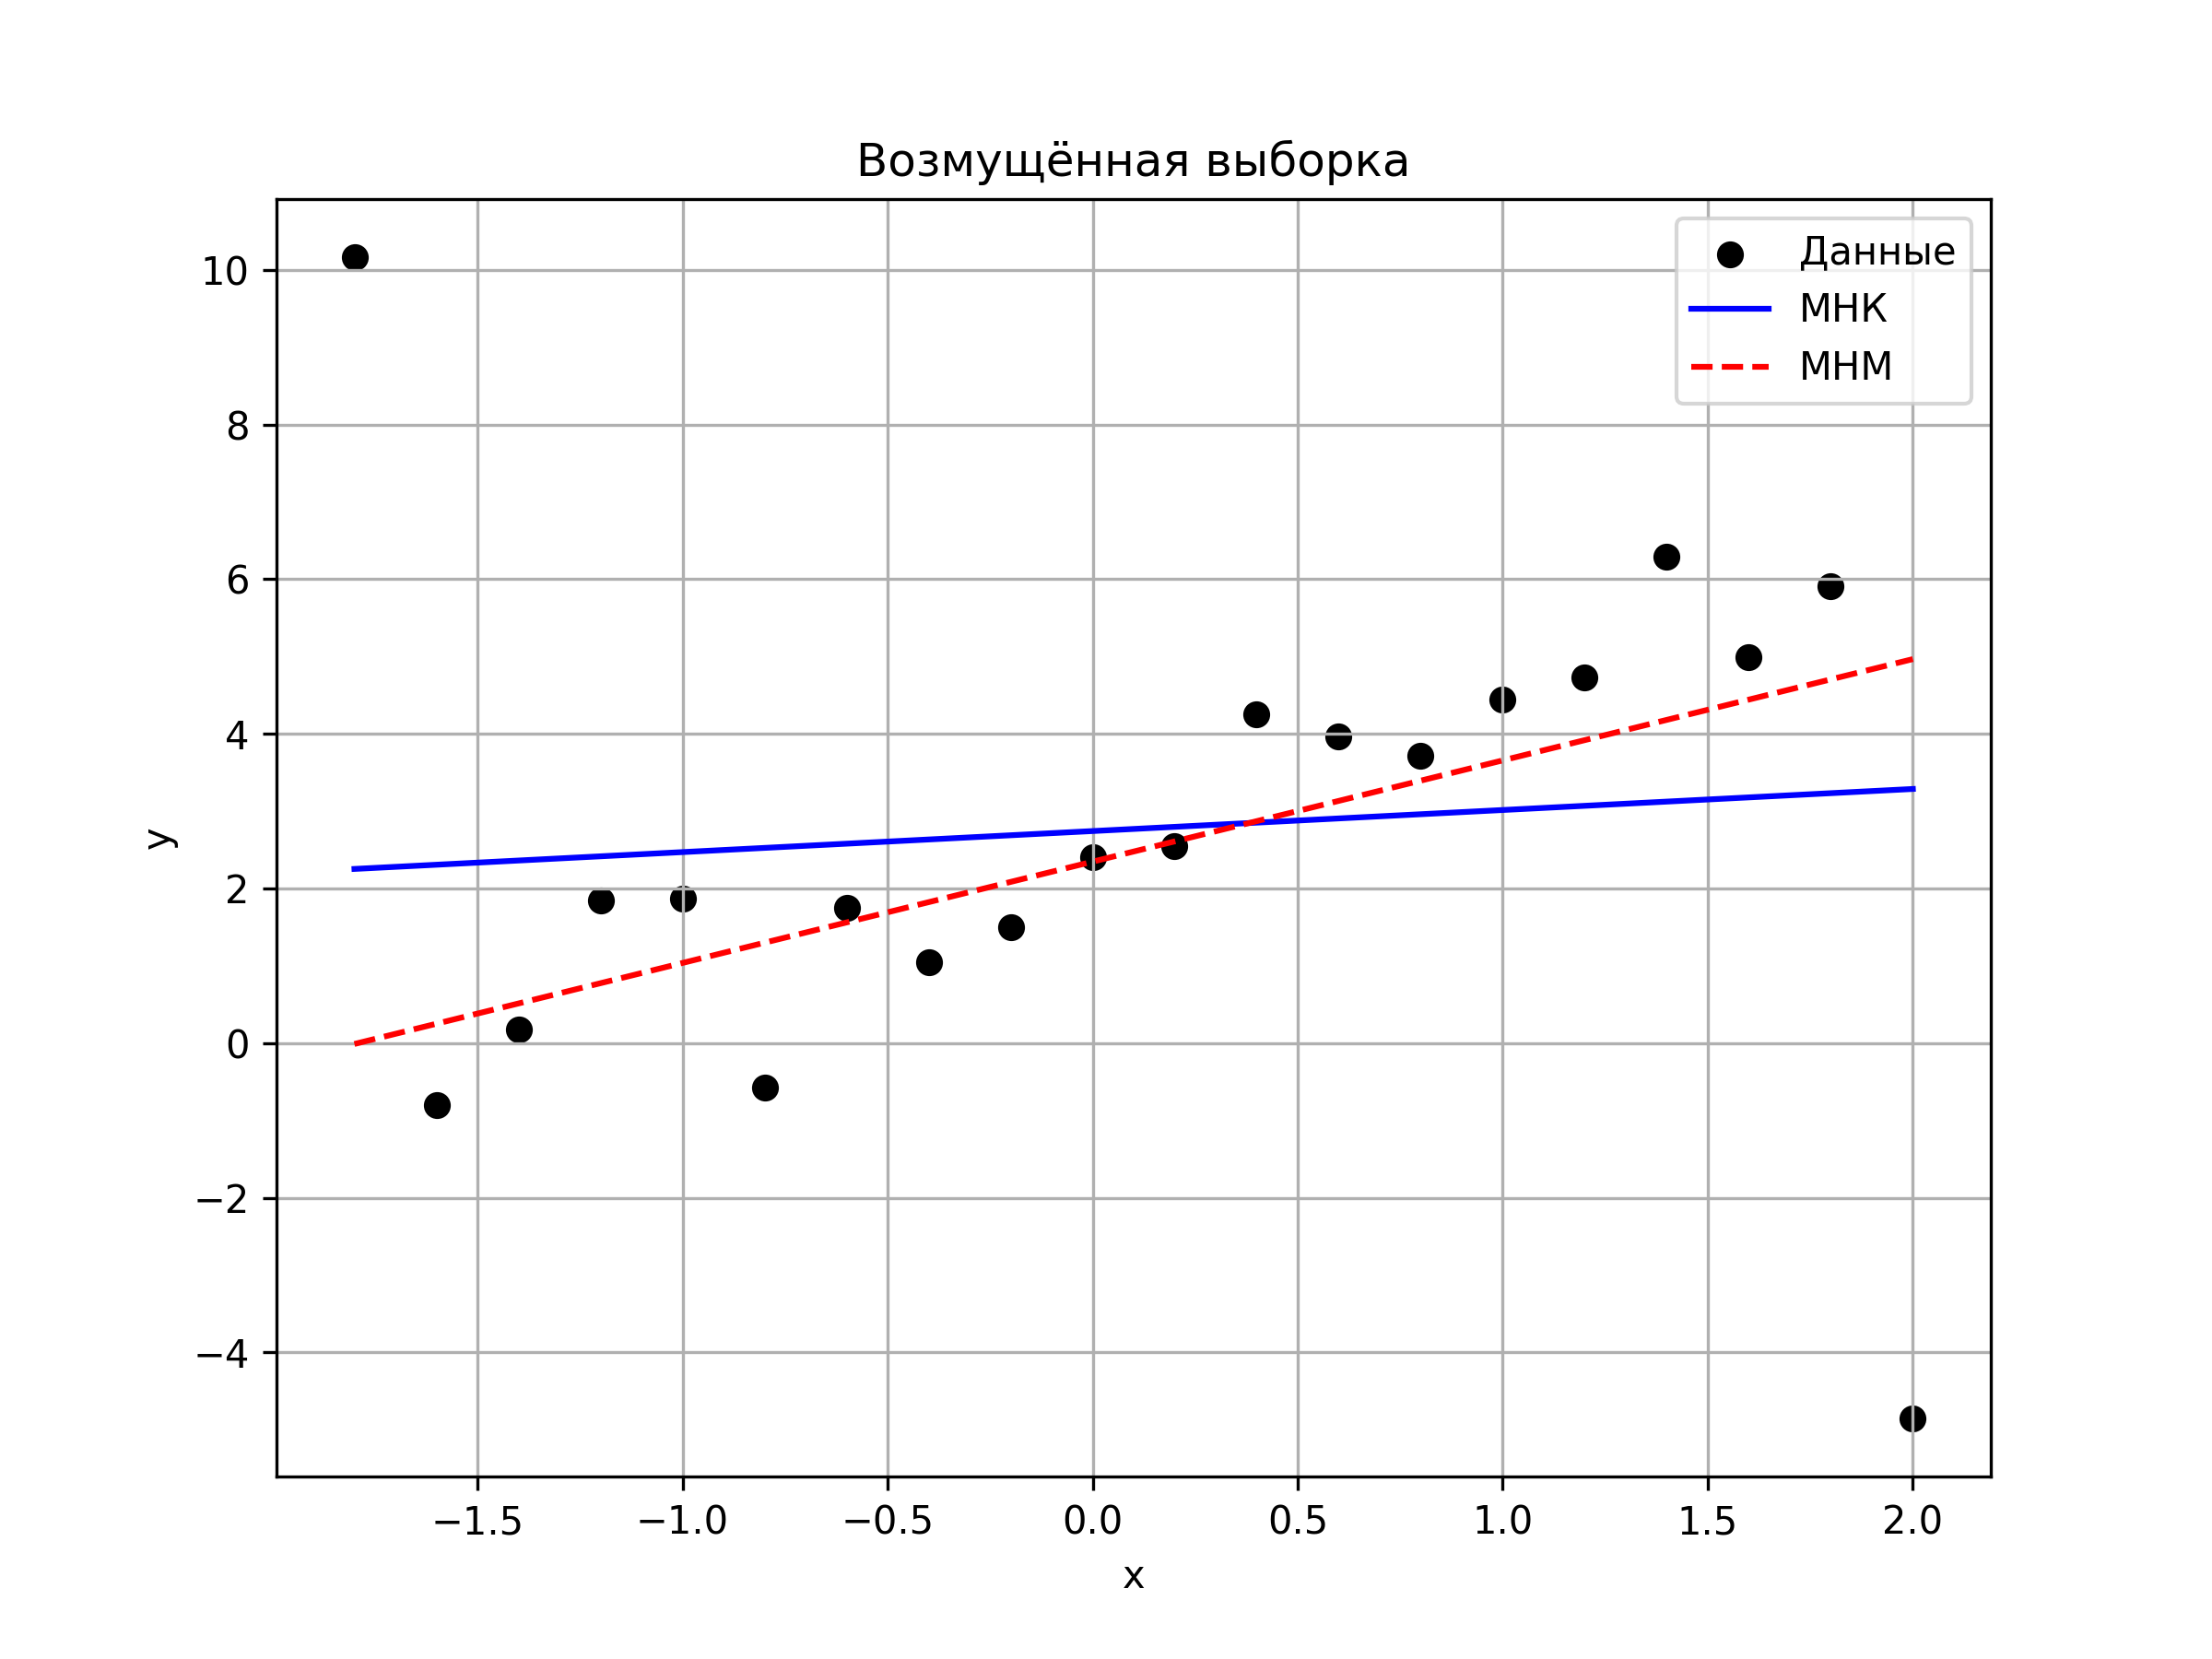
\includegraphics[width=0.8\textwidth]{regression_perturbed}
        \caption{Возмущённая выборка: влияние выбросов}
    \end{figure}


    \section{Выводы}

    \begin{itemize}
        \item Метод наименьших квадратов (МНК) показывает хорошие результаты на "чистых" данных, но чувствителен к выбросам.
        \item Метод наименьших модулей (МНМ) демонстрирует устойчивость к возмущениям в данных, хоть и менее точен в случае нормальных данных без выбросов.
        \item Графики подтверждают, что линия регрессии, построенная МНК, сильно смещается при наличии выбросов, в то время как линия МНМ остаётся близкой к истинной зависимости.
    \end{itemize}


\end{document}